\documentclass[aps,pre,twocolumn,superscriptaddress,floatfix]{revtex4-2}
\usepackage{amsmath,amssymb,amsfonts,graphicx,bm}
\usepackage{hyperref}

\begin{document}

\title{The Dimensional Work of Surfaces: A Thermodynamic Origin of Minimal Geometry and Surface Tension}

\author{Ian Todd}
\email{itod2305@uni.sydney.edu.au}
\affiliation{Sydney Medical School, University of Sydney, Sydney, NSW 2006, Australia}

\date{\today}

\begin{abstract}
Surface tension and minimal surfaces play central roles across soft matter physics, geometry, and biological interfaces. Classical theory describes interfaces through geometric energy functionals such as $\gamma A$, the Young--Laplace law, and Helfrich curvature elasticity. Yet the thermodynamic origin of these geometric energies remains opaque: why does curvature cost energy, and what principle underlies the drive toward minimal geometry?

Here we show that the geometric energetics of surfaces emerge naturally from the \emph{Dimensional Landauer Bound}, which generalizes Landauer's principle to high-dimensional dynamical systems constrained to low-dimensional manifolds. When a noisy physical system is confined to a two-dimensional interface embedded in three dimensions, the minimum work required to impose that constraint is $W_{\mathrm{dim}} = k_B T \, C_\Phi$, where $C_\Phi = D_{\mathrm{KL}}(p(x)\,\Vert\,\Phi^\dagger p(y))$ is a KL-based \emph{dimensional contraction cost}. For smooth surfaces $\Phi(u,v)$, we show that this reduces to a functional of the induced metric:
\[
W_{\mathrm{dim}} \;\propto\; k_B T \int \log\sqrt{\det G(u,v)} \, p(u,v)\,du\,dv,
\]
with $G = J_\Phi J_\Phi^\top$ the first fundamental form. Expanding this functional yields curvature-dependent terms identical to classical surface energies: area minimization, mean curvature flow, and the Young--Laplace pressure. Surface tension thus appears not as a primitive constant, but as the thermodynamic cost of constraining high-dimensional stochastic fluctuations onto a curved two-dimensional manifold.

We validate this perspective through simulation of a Brownian particle confined to a fluctuating surface. The \emph{maintenance power} required to sustain confinement decreases monotonically as the surface relaxes toward minimal geometry, mirroring soap film relaxation under surface tension. Just as the Dimensional Landauer Bound distinguishes formation cost (work to create a state) from maintenance cost (power to sustain it), surface tension represents the geometric free energy while dissipation measures the dynamic cost of preserving that geometry against noise.
\end{abstract}

\maketitle

%------------------------------------------------------------------------------
\section{Introduction}
%------------------------------------------------------------------------------

Interfaces and surfaces are ubiquitous in physical and biological systems. Soap films, lipid membranes, cell boundaries, and emulsion droplets are all controlled by the energetics of curvature. Classical approaches model these systems via geometric energy functionals: surface tension $E = \gamma A$, the Young--Laplace law $\Delta P = 2\gamma H$, and Helfrich bending elasticity $E = \int [\gamma + \frac{\kappa}{2}(2H)^2]\,dA$~\cite{helfrich1973,safran1994}. However, these expressions are typically postulated as continuum energy functionals, not derived from a more general thermodynamic principle.

In recent work, the \emph{Dimensional Landauer Bound} was introduced to describe the energetic cost of constraining a high-dimensional stochastic system to a lower-dimensional manifold~\cite{todd2025landauer}. The bound states that the minimum work required to impose a dimensional reduction $\Phi:\mathbb{R}^{D_{\mathrm{in}}}\to\mathbb{R}^{D_{\mathrm{out}}}$ is
\begin{equation}
W_{\mathrm{dim}} = k_B T \, D_{\mathrm{KL}}(p(x)\,\Vert\,\Phi^\dagger p(y)),
\label{eq:dim_landauer}
\end{equation}
where $p(x)$ is the true distribution of microscopic states, $p(y)$ is the induced distribution on the lower-dimensional manifold, and $\Phi^\dagger p(y)$ is the maximum-entropy lift back into the full space.

In this paper, we apply this framework to smooth surfaces and show that classical surface energetics arise as the \emph{dimensional work} required to constrain microscopic fluctuations to a curved two-dimensional manifold embedded in three dimensions. We derive continuum expressions for $W_{\mathrm{dim}}$ in terms of the induced metric and curvature, recover standard surface tension and Helfrich energies, and illustrate the resulting principle in a simple soap-film-like simulation.

%------------------------------------------------------------------------------
\section{Dimensional Work for Smooth Surfaces}
%------------------------------------------------------------------------------

\subsection{Surface embedding and induced metric}

Consider a smooth surface embedded in $\mathbb{R}^3$,
\begin{equation}
\Phi(u,v): \Omega \subset \mathbb{R}^2 \to \mathbb{R}^3.
\end{equation}
We regard $(u,v)$ as internal coordinates and $\Phi(u,v)$ as the embedding. The Jacobian of $\Phi$ is
\begin{equation}
J_\Phi(u,v) =
\begin{pmatrix}
\partial_u \Phi \\[3pt]
\partial_v \Phi
\end{pmatrix},
\end{equation}
and the induced metric (first fundamental form) is
\begin{equation}
G(u,v) = J_\Phi(u,v) J_\Phi(u,v)^\top.
\end{equation}
The local area element of the surface is $dA = \sqrt{\det G(u,v)}\,du\,dv$.

\subsection{KL-based dimensional work in the continuum limit}

Following the Dimensional Landauer framework, we consider a high-dimensional stochastic process $X_t$ in $\mathbb{R}^3$ with distribution $p(x)$, constrained to remain near the surface $\Phi(u,v)$. Let $p(u,v)$ denote the induced distribution on the surface coordinates, and let $\Phi^\dagger p(u,v)$ be the corresponding lifted distribution on $\mathbb{R}^3$ that is maximally uninformative orthogonal to the surface.

The dimensional contraction cost is then
\begin{equation}
C_\Phi = D_{\mathrm{KL}}\big(p(x)\,\Vert\,\Phi^\dagger p(u,v)\big).
\end{equation}
Under mild regularity assumptions and for fluctuations narrow around the surface, this KL divergence admits the approximation
\begin{equation}
C_\Phi \;\approx\; \int_\Omega \log\sqrt{\det G(u,v)} \, p(u,v)\,du\,dv.
\label{eq:Cphi_surface}
\end{equation}

\subsection{Area functional and surface tension}

In the simplest case where $p(u,v)$ is approximately uniform over a patch of the surface, Eq.~\eqref{eq:Cphi_surface} reduces to an integral over the log-determinant. For small deviations from a flat reference, we may expand $\log\sqrt{\det G} \approx \sqrt{\det G} - 1 + \mathcal{O}((\nabla\Phi)^2)$, yielding
\begin{equation}
W_{\mathrm{dim}} \approx \gamma \int_\Omega \sqrt{\det G(u,v)}\,du\,dv = \gamma A,
\end{equation}
where $A$ is the surface area and $\gamma$ is an effective surface tension parameter proportional to $k_B T$. Thus, the classical surface tension energy $\gamma A$ appears as the leading contribution to dimensional work.

\subsection{Young--Laplace law from variational principle}

If we consider a normal variation $\Phi \to \Phi + \epsilon \eta n$, where $n$ is the unit normal and $\eta$ is a scalar field on the surface, the first variation of area is~\cite{docarmo1976}
\begin{equation}
\delta A = -2 \int_\Sigma H \eta\, dA,
\end{equation}
where $H$ is the mean curvature. Extremizing dimensional work under a volume constraint $\delta V = \int_\Sigma \eta\,dA$ with Lagrange multiplier $\Delta P$ yields
\begin{equation}
\Delta P = 2\gamma H,
\end{equation}
which is the Young--Laplace equation. In this view, Laplace pressure is the Lagrange multiplier enforcing volume conservation in the presence of dimensional work proportional to area.

\subsection{Helfrich curvature elasticity}

Higher-order terms in the expansion of $\log\sqrt{\det G}$ generate curvature-dependent contributions. Retaining second-order terms yields a bending energy of the form
\begin{equation}
W_{\mathrm{dim}} \approx \gamma \int dA + \kappa \int (2H)^2\,dA + \cdots,
\end{equation}
which matches the Helfrich Hamiltonian used to model lipid bilayers~\cite{helfrich1973}. Thus, both surface tension and curvature elasticity emerge as different orders of dimensional work.

%------------------------------------------------------------------------------
\section{Mean Curvature Flow as Gradient Descent}
%------------------------------------------------------------------------------

The gradient of dimensional work with respect to the embedding is
\begin{equation}
\frac{\delta W_{\mathrm{dim}}}{\delta \Phi} = -2\gamma H \, n.
\end{equation}
A natural dissipative evolution that reduces dimensional work most rapidly is gradient flow:
\begin{equation}
\frac{\partial \Phi}{\partial t} = -M \frac{\delta W_{\mathrm{dim}}}{\delta \Phi} = 2M\gamma H\, n.
\end{equation}
After rescaling time, this is exactly the \textbf{mean curvature flow} equation:
\begin{equation}
\frac{\partial \Phi}{\partial t} = H\, n,
\end{equation}
which describes the relaxation of soap films and interfaces toward minimal surfaces~\cite{brakke1978}. Stationary points satisfy $H = 0$---minimal surfaces are precisely the zero-dimensional-work geometries.

%------------------------------------------------------------------------------
\section{Simulation: Maintenance Power and Surface Geometry}
%------------------------------------------------------------------------------

To illustrate the dynamic consequences of geometric free energy, we consider a Brownian particle in 3D constrained to remain near a surface
\begin{equation}
z = f(x,y; A) = A \sin x \sin y,
\end{equation}
where amplitude $A$ controls roughness and curvature. The particle obeys overdamped Langevin dynamics with a harmonic confinement potential $U_{\mathrm{conf}} = \frac{k}{2}[z - f(x,y;A)]^2$.

We measure the \emph{maintenance power}---the continuous dissipation required to sustain confinement against thermal fluctuations---using $\langle|\mathbf{F}_{\mathrm{conf}}|^2\rangle$ as a power proxy (see Appendix~\ref{app:sim}).

Figure~\ref{fig:surface} shows that as $A$ decreases from a highly wavy surface toward the flat minimal configuration ($A \to 0$), the maintenance power decreases monotonically. This numerically confirms that \emph{surfaces with lower geometric free energy require less power to maintain}. The maintenance power scales with the same geometric parameters (curvature, metric distortion) that determine the formation cost $W_{\mathrm{dim}}$, validating the Dimensional Landauer framework in the surface setting.

\begin{figure}[t]
\centering
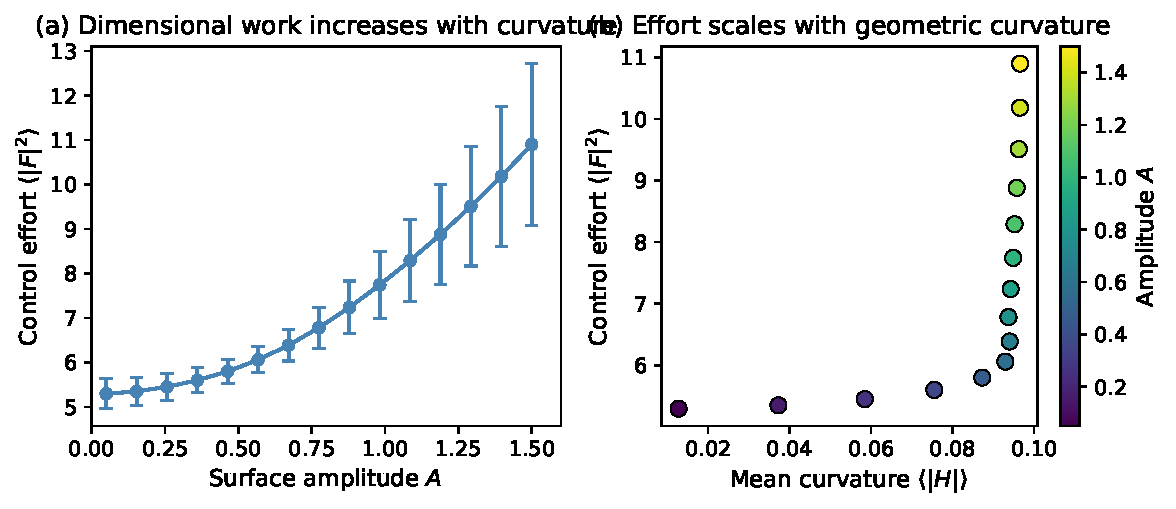
\includegraphics[width=\columnwidth]{figures/fig1_surface_work.pdf}
\caption{\textbf{Maintenance power decreases with geometric complexity.} Mean maintenance power for confining a Brownian particle to a surface $z = A\sin x\sin y$ as a function of amplitude $A$. As the surface flattens ($A \to 0$), maintenance power decreases monotonically, paralleling the decrease in geometric free energy (surface tension) during soap film relaxation.}
\label{fig:surface}
\end{figure}

%------------------------------------------------------------------------------
\section{Discussion}
%------------------------------------------------------------------------------

We have shown that the geometric energetics of classical surfaces---surface tension, Laplace pressure, and curvature elasticity---emerge naturally from the dimensional work term of the Dimensional Landauer Bound. Constraining microscopic fluctuations to remain on or near a curved interface requires continuous suppression of degrees of freedom orthogonal to the surface.

This framework distinguishes two complementary costs. The \emph{formation cost} $W_{\mathrm{dim}} = \gamma A$ is the free energy required to establish a surface---analogous to the ``deposit'' for creating geometric structure. The \emph{maintenance cost} is the continuous power dissipation required to sustain that structure against thermal fluctuations---the ``rent'' that must be paid to preserve low-dimensional geometry. Our simulations measure maintenance power, which scales with the same geometric parameters (curvature, area) that determine formation cost.

This yields a unified interpretation: curvature costs energy because it imposes a stricter constraint on accessible microscopic configurations. Minimal surfaces arise as configurations that minimize dimensional work. Mean curvature flow is the gradient descent of this thermodynamic functional.

While classical surface tension arises from intermolecular forces, our framework reveals a purely entropic component scaling as $k_B T$ that exists for any fluctuating interface, even in the absence of cohesive forces. This entropic contribution is the irreducible cost of dimensional confinement itself.

Notably, Gaussian curvature does not appear in the dimensional work functional because it integrates to a topological invariant (Gauss--Bonnet theorem) and cannot affect shape variations for fixed topology. This is consistent with classical capillarity where only mean curvature enters the energetics.

Beyond classical capillarity, this principle may apply broadly to biological membranes, active matter interfaces, and shape control in living systems. It also suggests a parallel between geometric variational principles in soft matter and representation learning in high-dimensional systems: in both cases, low-dimensional manifolds arise as compromise solutions minimizing an underlying dimensional work functional.

\begin{acknowledgments}
The author thanks the Sydney Medical School for support and members of the Fulcher Lab at the University of Sydney for discussions on dimensionality and thermodynamics.
\end{acknowledgments}

\appendix

%------------------------------------------------------------------------------
\section{Derivation of Area and Curvature Terms}
\label{app:derivation}
%------------------------------------------------------------------------------

In this appendix we outline the derivation of geometric energies from the KL-based dimensional work functional.

\subsection{Expansion of the log-determinant}

Let $\sqrt{\det G} = 1 + \epsilon(u,v)$, where $\epsilon$ measures deviation from flatness. Expanding the logarithm,
\begin{equation}
\log(1+\epsilon) = \epsilon - \tfrac{1}{2}\epsilon^2 + \mathcal{O}(\epsilon^3),
\end{equation}
we obtain
\begin{equation}
C_\Phi \approx \int_\Omega \epsilon\, p(u,v)\,du\,dv - \frac{1}{2}\int_\Omega \epsilon^2\, p(u,v)\,du\,dv + \cdots
\end{equation}

To first order, $C_\Phi^{(1)} \propto \int_\Omega \sqrt{\det G}\,du\,dv = A$, the total surface area. Thus, the leading contribution to $W_{\mathrm{dim}}$ is $W_{\mathrm{dim}}^{(1)} = \gamma A$, with $\gamma \propto k_B T$ an effective surface tension.

\subsection{Variation of area and Young--Laplace}

Under a normal displacement $\Phi \to \Phi + \epsilon\eta n$, the first variation of area is
\begin{equation}
\delta A = -2\int_\Sigma H\eta\,dA.
\end{equation}
If $W_{\mathrm{dim}}^{(1)} = \gamma A$, then $\delta W_{\mathrm{dim}}^{(1)} = -2\gamma\int_\Sigma H\eta\,dA$.

Imposing volume conservation with Lagrange multiplier $\Delta P$ and using $\delta V = \int_\Sigma \eta\,dA$, we obtain $-2\gamma H - \Delta P = 0$, yielding the Young--Laplace equation $\Delta P = 2\gamma H$.

\subsection{Second-order terms and curvature elasticity}

In the small-gradient approximation $\Phi(x,y) = (x,y,h(x,y))$, the area element expands as $\sqrt{\det G} \approx 1 + \frac{1}{2}|\nabla h|^2 + \cdots$, and mean curvature is $H \approx \frac{1}{2}\nabla^2 h + \mathcal{O}(|\nabla h|^2)$.

The second-order term $\int \epsilon^2\,dA$ can be rewritten as $\int H^2\,dA$, yielding an effective bending energy $W_{\mathrm{dim}}^{(2)} = \kappa\int(2H)^2\,dA$, analogous to Helfrich curvature elasticity.

%------------------------------------------------------------------------------
\section{Mean Curvature Flow as Gradient Descent}
\label{app:mcf}
%------------------------------------------------------------------------------

The gradient of dimensional work with respect to the embedding is
\begin{equation}
\frac{\delta W_{\mathrm{dim}}}{\delta \Phi} = -2\gamma H\,n.
\end{equation}
Gradient flow dynamics $\partial_t\Phi = -M\,\delta W_{\mathrm{dim}}/\delta\Phi$ yield
\begin{equation}
\frac{\partial\Phi}{\partial t} = 2M\gamma H\,n.
\end{equation}
After rescaling time, this is the mean curvature flow equation $\partial_t\Phi = H\,n$, which describes soap film relaxation toward minimal surfaces~\cite{brakke1978}.

Stationary points satisfy $H = 0$, corresponding to minimal surfaces. Thus:
\begin{quote}
\textbf{Mean curvature flow is the gradient descent of dimensional work.}
\end{quote}

Minimal surfaces are precisely the zero-dimensional-work geometries (to leading order).

%------------------------------------------------------------------------------
\section{Gaussian Curvature and Topology}
\label{app:gauss}
%------------------------------------------------------------------------------

Gaussian curvature $K$ does not appear in the dimensional work functional. This is not a deficiency but a consequence of the Gauss--Bonnet theorem:
\begin{equation}
\int_\Sigma K\,dA = 2\pi\chi(\Sigma),
\end{equation}
where $\chi(\Sigma)$ is the Euler characteristic, a topological invariant.

Since $\int K\,dA$ is independent of geometry for fixed topology, variations vanish:
\begin{equation}
\frac{\delta}{\delta\Phi}\int_\Sigma K\,dA = 0.
\end{equation}

The KL contraction cost depends on local volume compression via $\log\sqrt{\det G}$, which is a function of the metric only. Gaussian curvature depends on the second fundamental form and is topologically protected.

Thus, the dimensional work functional correctly produces surface tension ($\gamma A$) and bending rigidity ($\kappa\int H^2\,dA$) while omitting topological terms, in exact agreement with classical capillarity.

%------------------------------------------------------------------------------
\section{Simulation Details}
\label{app:sim}
%------------------------------------------------------------------------------

We simulated a Brownian particle in 3D confined to a surface $z = A\sin x\sin y$ with amplitude $A$ controlling curvature. The particle obeys overdamped Langevin dynamics:
\begin{equation}
\dot{\mathbf{r}}_t = -\nabla U_{\mathrm{conf}}(\mathbf{r}_t) + \sqrt{2D}\,\bm{\eta}_t,
\end{equation}
with confinement potential $U_{\mathrm{conf}} = \frac{k}{2}[z - f(x,y;A)]^2$, diffusion coefficient $D = 0.1$, and stiffness $k = 50$.

Maintenance power was measured as $\langle|\mathbf{F}_{\mathrm{conf}}|^2\rangle$, the mean squared confinement force, which is proportional to the dissipation rate in a viscous medium. This quantity measures the continuous power required to sustain the particle's confinement against thermal fluctuations---the dynamic ``rent'' for maintaining a low-dimensional state. Simulations used $\Delta t = 10^{-3}$, $N = 8000$ steps, and 5 independent trials per amplitude.

Results (Fig.~\ref{fig:surface}) show maintenance power increasing monotonically with amplitude: from $\sim 5.3$ at $A = 0.05$ (nearly flat) to $\sim 10.9$ at $A = 1.5$ (highly curved). This confirms that surfaces with higher geometric free energy (larger $W_{\mathrm{dim}}$) require proportionally higher maintenance power, validating the scaling predicted by the Dimensional Landauer framework.

\bibliography{references}

\end{document}
